\clearpage
\section{Statistical Analysis}
\subsection{Mode selection}
With large datasets, previous "event display" method will no longer be efficient and accurate. Thus data analysis tools are necessary. Here \verb|root| is used and three macros to apply cuts are already implemented. As before we have four sets of Monte Carlo simulated data in order to find the optimal cuts, then there are a couple of real data samples.

First of all, there are a couple of general cuts. The collider energy of LEP is $\sim\SI{200}{\giga\eV}$. Thus the scalar sum of momenta should be maximally around this value. Events with even larger momenta are caused by various unphysical processes. Secondly, the data here is written such as when there are multiple outgoing positive particles, $\verb|cos_thet|=1000$. For $ee$ and $\mu\mu$ process, it should not be possible, since no hadronisation can occur and initial/final state radiation for these two only involve photons. So for these two event selections, cut $\verb|cos_thet| <= 1.0$ is applied, see figure~\ref{fig:cos_thet_cut}. After the cut(s), there are $56613$ $ee$ events, $89646$ $\mu\mu$ events, $79099$ $\tau\tau$ events, and $98100$ $qq$ events.
\begin{figure}[ht]
	\centering
	\includegraphics[width=0.8\linewidth]{cos_thet_before.pdf}
	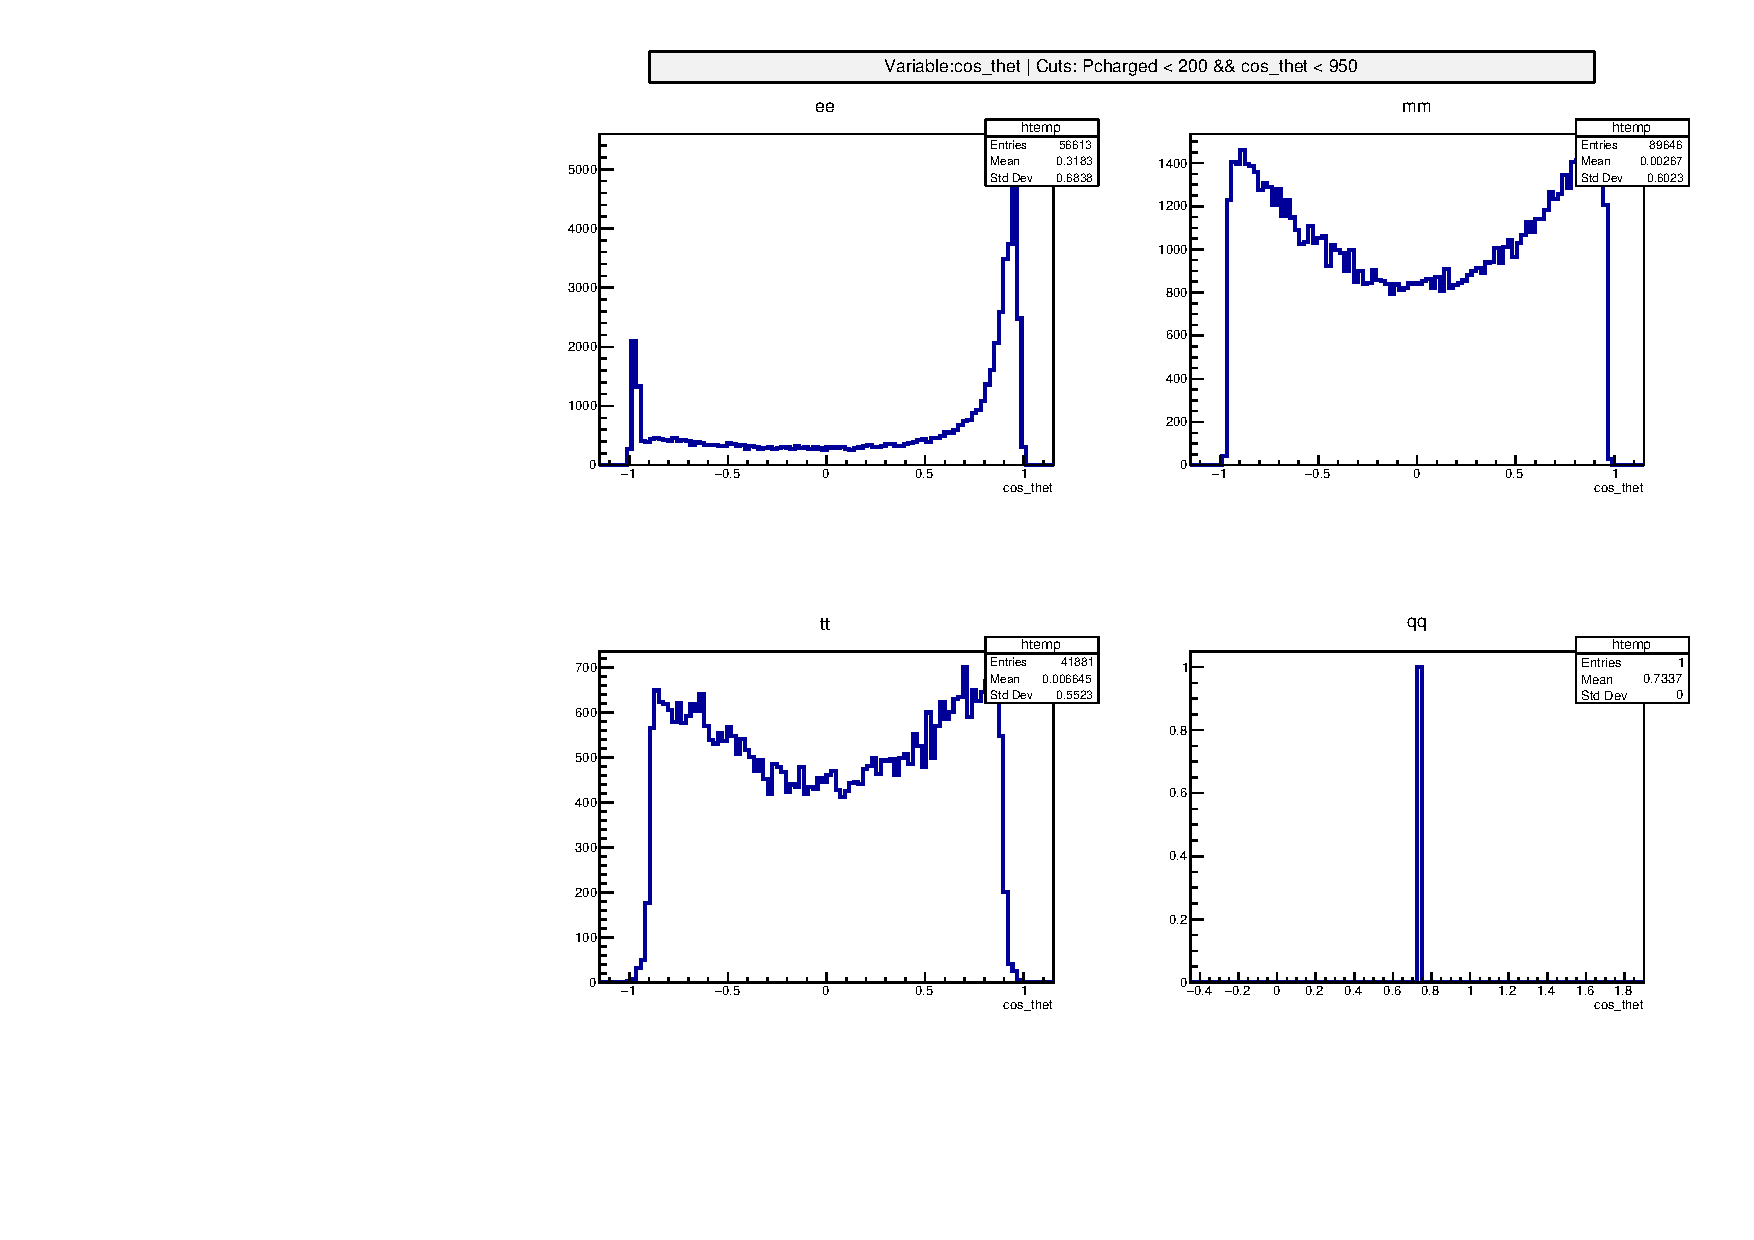
\includegraphics[width=0.8\linewidth]{cos_thet_after.pdf}
	\cprotect\caption{Distribution of \verb|cos_thet| before and after \verb|cos_thet| cut.}%
	\label{fig:cos_thet_cut}
\end{figure}

\clearpage
In event display part, we had success using cut $\verb|Ncharged| > 7$ for $qq$ processes. We conclude that this is no longer sufficient, since there are quite many $\tau\tau$ contamination, see figure~\ref{fig:qq_Ncharged_cuts}. While roughly $5\%$ percent of $qq$ events are lost, $\tau\tau$ events are barely present and $ee$, $\mu\mu$ are completely cut. So the $5\%$ percent are considered as acceptable "casualties". After the cut for $qq$, no $ee$ or $\mu\mu$ are left, $78$ $\tau\tau$ survives and $92688$ $qq$ events remain.
\begin{figure}[ht]
	\centering
	\includegraphics[width=0.8\linewidth]{N_charged_before2.pdf}
	\includegraphics[width=0.8\linewidth]{N_charged_after.pdf}
	\cprotect\caption{Number of charged tracks (\verb|Ncharge|) before and after the refined cut for $qq$ events.}%
	\label{fig:qq_Ncharged_cuts}
\end{figure}

Follow the same receipt as in event display part, we try to separate $ee$ events from other leptonic channels. Cut in number of charged track remains the same: $\verb|Ncharged| < 4 $ or ($\leq 3$). Same as before \verb|E_ecal| of $ee$ events have peak at around \SI{80}{\giga\eV}. \verb|E_ecal| cut is changed to $\verb|E_ecal| > 60$, since there is virtually no events even at $\verb|E_ecal| = 60$, see figure~\ref{fig:ee_cuts}. \verb|E_hcal| cut is similar to before, just relaxed a little bit (to \verb|E_hcal < 2|), since some of events have higher \verb|E_hcal| as previous cut, see figure~\ref{fig:ee_cuts_hcal}. In the end, we end up with $51679$ $ee$ events, $0$ $\mu\mu$, $910$ $\tau\tau$ events, and $1$ $qq$ event.
\begin{figure}[ht]
	\centering
	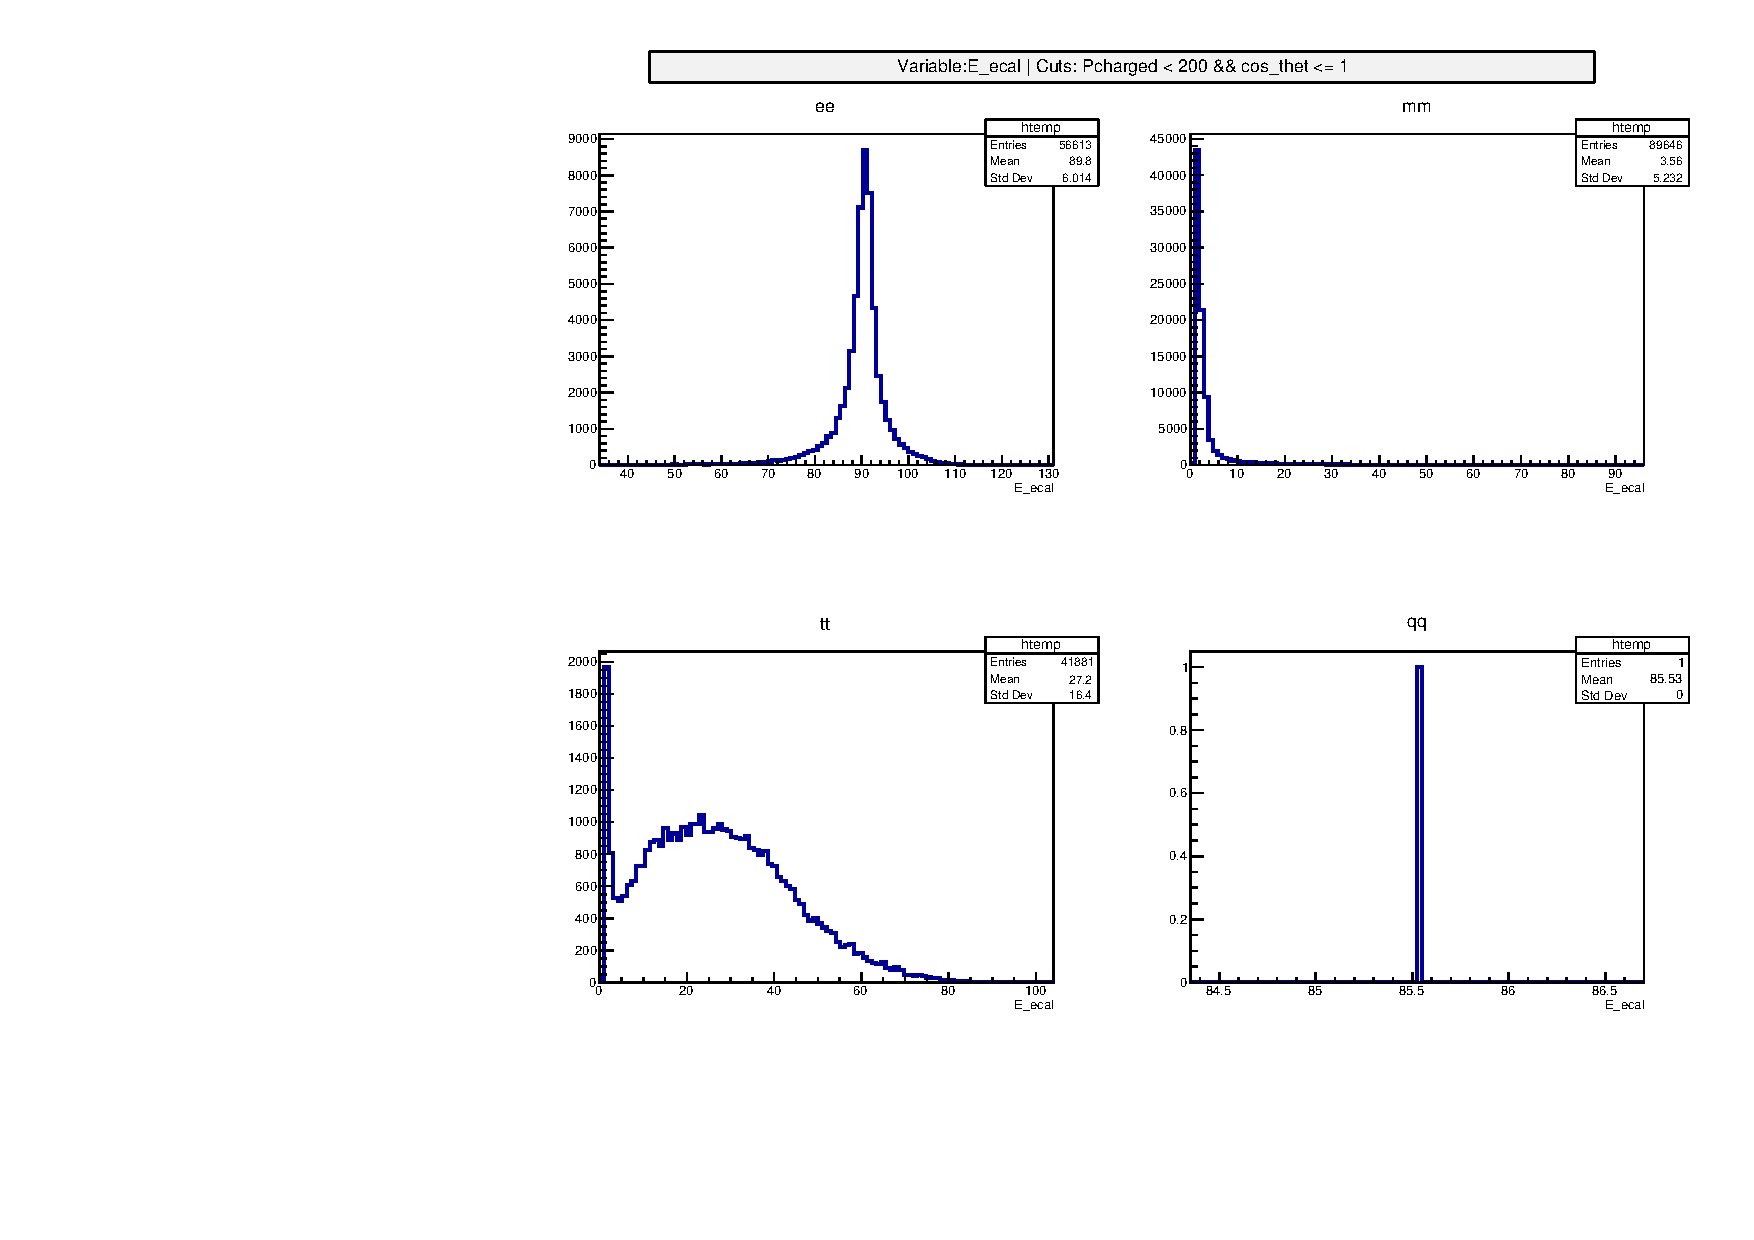
\includegraphics[width=0.8\linewidth]{ecal_before_ecal_cut.pdf}
	\cprotect\caption{\verb|E_ecal| distribution before \verb|E_ecal| cut for $ee$. }%
	\label{fig:ee_cuts}
\end{figure}
\begin{figure}[ht]
	\centering
	\includegraphics[width=0.8\linewidth]{hcal_after_Ncharged_ecal_cuts.pdf}
	\cprotect\caption{\verb|E_hcal| distribution after \verb|E_ecal| but before \verb|E_hcal| cut for $ee$.}%
	\label{fig:ee_cuts_hcal}
\end{figure}


For $\mu\mu$ selection, cut in \verb|Ncharged| is the same as $ee$: $\verb|Ncharged < 4|$. We have already seen in figure~\ref{fig:ee_cuts} that \verb|E_ecal| of $\mu\mu$ has a peak around $0$, so the \verb|E_ecal| cut for $ee$ gets inverted as cut for $\mu\mu$: $\verb|E_ecal| < 60$. Then remaining $\tau\tau$ events can be excluded with the help of \verb|Pcharged|, see figure~\ref{fig:mm_cuts}. $ee$ and $qq$ events are basically cut away, only unwanted events are $\tau\tau$. \verb|Pcharged| distributions of $\mu\mu$ and $\tau\tau$ are separated quite nicely, although some $\mu\mu$ events have $\verb|Pcharged| \approx 0$. A cut at $\verb|Pcharged| > 70$ will remove most of $\tau\tau$ events while preserve most of $\mu\mu$ events. After combinations of these cuts, $144$ $ee$ events, $83228$ $\mu\mu$ events, $480$ $\tau\tau$ events and zero $qq$ event survive.
\begin{figure}[ht]
	\centering
	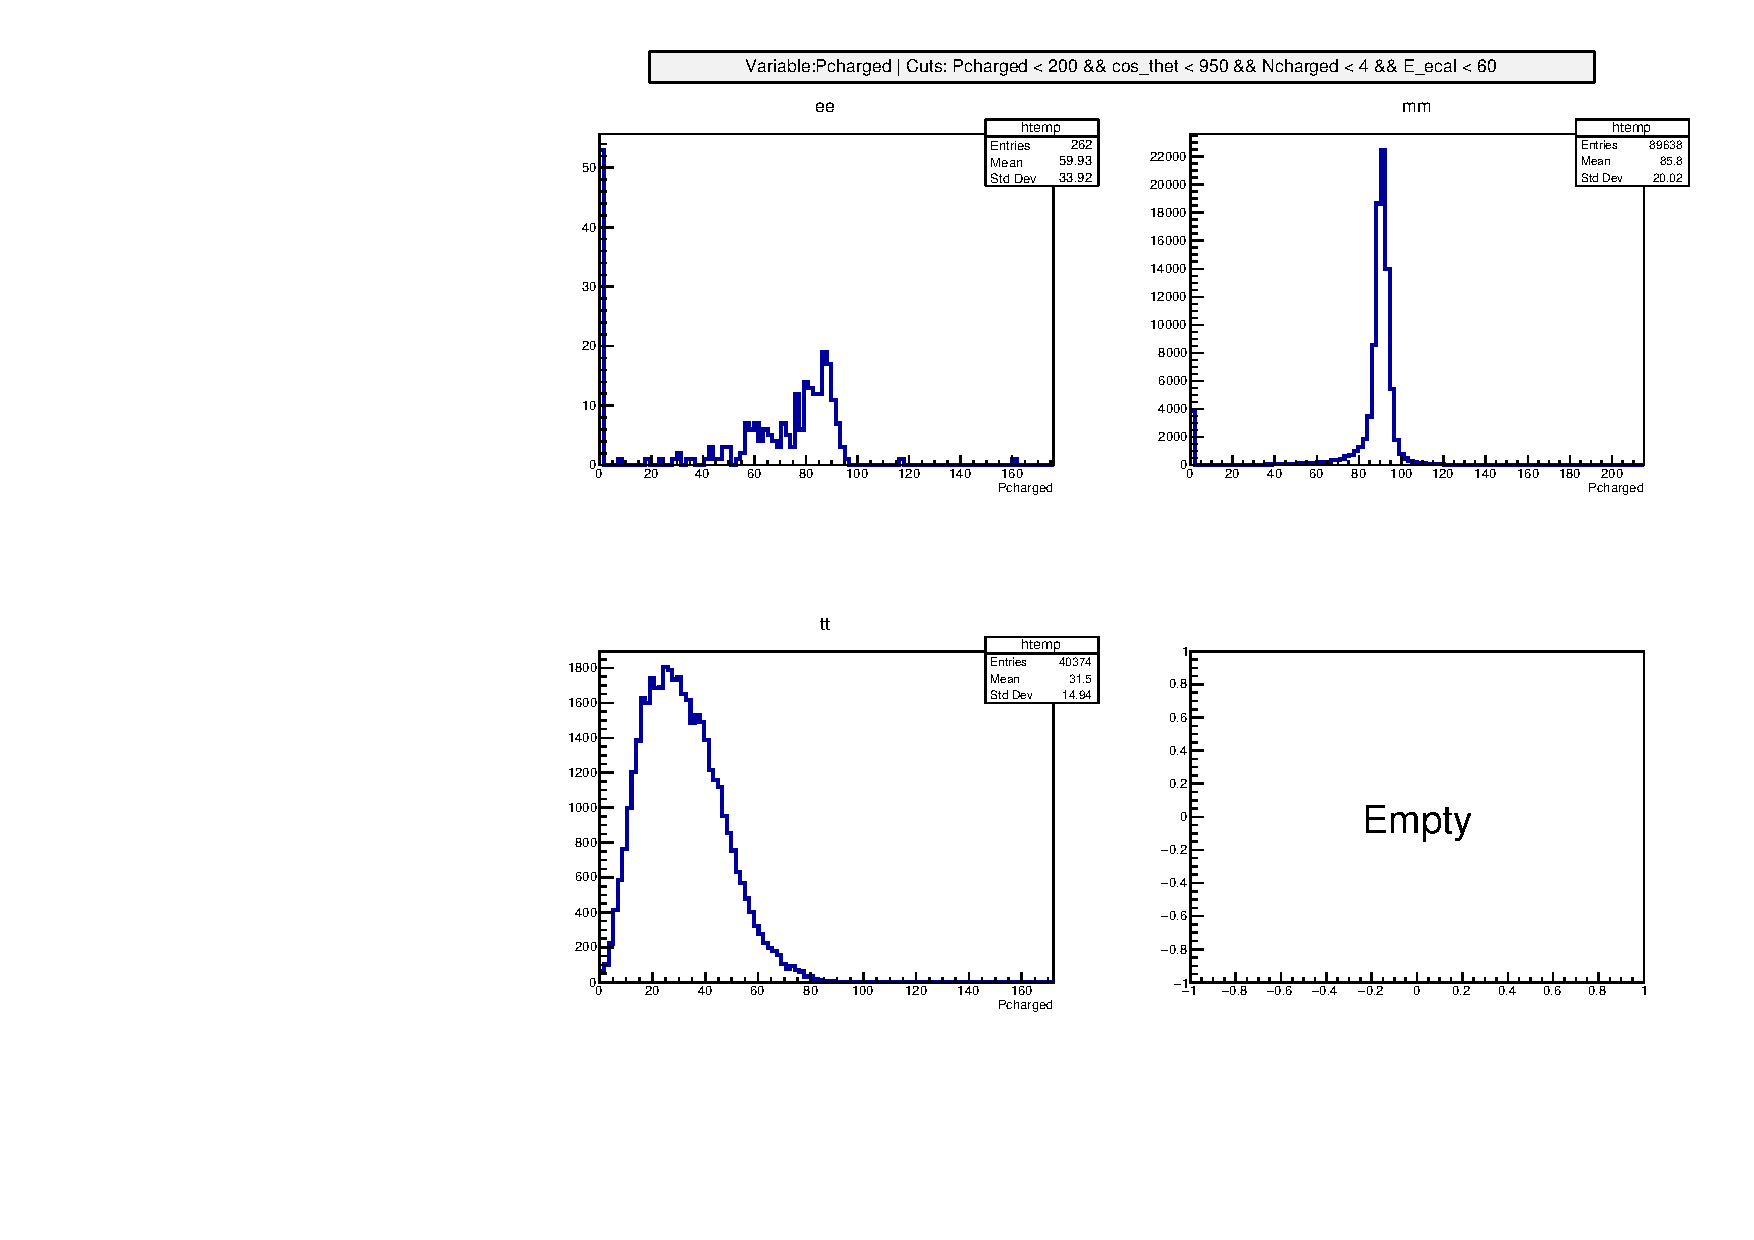
\includegraphics[width=0.8\linewidth]{Pcharged_mm_before_pcharged_cut.pdf}
	\cprotect\caption{\verb|Pcharged| distribution after \verb|E_ecal| cut for $\mu\mu$.}%
	\label{fig:mm_cuts}
\end{figure}

$\tau\tau$ can be picked out using the same cuts for $\mu\mu$ expect $\verb|Pcharged|$ cut gets inverted. Since there is a small peak at $\verb|Pcharged| = 0$ in $ee$ and $\mu\mu$ events, see figure~\ref{fig:mm_cuts}, a lower bound in \verb|Pcharged| should be set as well. Thus for $\mu\mu$: $1< \verb|Pcharged| < 60$. $E_ecal$ cut should be adjusted a bit. In figure~\ref{fig:ee_cuts}, there are still quite substantial amount of $\tau\tau$ event between $60 < \verb|E_ecal| < 70$. Thus we have for $\tau\tau$: $\verb|E_ecal| < 70$. Cut in \verb|Ncharged| is relaxed to $<5$ for better efficiency. After all these cuts, we have $243$ $ee$ events, $1446$ $\mu\mu$ events, $66990$ $\tau\tau$ events, and $38$ $qq$ events.

All the cuts are summarizes in table~\ref{tab:cuts_all}
\begin{table}[ht]
	\centering
	\begin{tabular}{cccccc}
		\toprule
	mode & \verb|cos_thet| & \verb|Pcharged| & \verb|Ncharged| & \verb|E_ecal| & \verb|E_hcal| \\
	\midrule
	$ee$ & $\leq 1$ & $< 200$ & $< 4$ & $>60$ & $< 2$ \\
	$\mu\mu$ & $\leq 1$ & $>70, <200$ & $<4$ & $<60$ & \\
	$\tau\tau$ & & $>1, <60$ & $<5$ & $<70$ \\
	$qq$ & & $<200$ & $>10$ & & \\
	\bottomrule
	\end{tabular}
	\caption{All cuts applied to select decay modes}
	\label{tab:cuts_all}
\end{table}

\clearpage
\subsection{Channel selection} Since processes with $e^+ e^-$ as final states include also $t$-channel elastic scattering between electron and positron and they are irrelevant processes in our discussion, we want to somehow get rid of these contributions. From figure~\ref{fig:angDep} in pre-lab tasks, we know that $s$-channel dominates at small $\cos\Theta$ and $s$-channel contributions should look like symmetric around $\cos\Theta = 0$. Naturally, first thing comes in our minds is to cut $\cos\Theta$ from somewhere between $0$ and $1$ to $-\infty$, so that it looks symmetric. Figure~\ref{fig:s_t_cut} is done with $\cos\Theta < 0.5$. There is a quite significant peak around $\cos\Theta = -1$, which we don't really expect. Physical origin of this peak is unknown to us, but anyway this should be cut away. In the end, we have the cut $-0.9 < \cos\Theta < 0.5$. This cut along with the previous $ee$ cuts will be the new $ee$ cuts used onwards.
\begin{figure}[ht]
	\centering
	\includegraphics[width=0.8\linewidth]{s_t_cut.pdf}
	\caption{$\cos\Theta$ distribution of $ee$ events after previously determined $ee$ cuts and $\cos \Theta< 0.5$.}%
	\label{fig:s_t_cut}
\end{figure}

\subsection{Forward-backward asymmetry}
Numbers of events in forward ($0 <\cos\theta<1$) and backward ($-1<\cos\theta<0$) are measured using \verb|data1.root| and MC data with $\mm$ as final states. In the actual analysis, only the real data are used. Upon inspection of definition~\ref{math:AFBdef}, it is clear that correction for cut efficiency is unnecessary here, since $N_{+,-}$ share the same cuts.

After application of equation~\ref{math:AFBdef} at all available CMS energy, correction terms should be added to the measured asymmetry. As we understand it, applying these corrections will remove radiation corrections in measured data, so that we can directly compare experimental values with tree-level theoretical values.
\begin{figure}[ht]
	\centering
	\includegraphics[width=0.8\linewidth]{A_FB.pdf}
	\caption{Forward-backward asymmetry after applying corrections. }%
	\label{fig:A_FB}
\end{figure}

Figure~\ref{fig:A_FB} shows the forward-backward asymmetry at various CMS energies. Errors are calculated as usual $\sigma_N \approx \sqrt{N}$.

If one says that the fourth data point (with $\sqrt{s} =\SI{91.22}{\giga\eV}$) lies \textit{exactly} at the peak of resonance, this $A_\text{FB}$ can be used to determined the Weinberg angle
\begin{align*}
	\sin^2\theta_W &= \frac{1-\sqrt{A^{\mu, \text{peak}}_{\text{FB}}/3}}{4} \\
	\sigma_{\sin^2\theta_W} &= \frac{1}{8\sqrt{3}} \frac{\sigma_A}{\sqrt{A}}	
\end{align*}
Then we have
\begin{equation}
	\sin^2\theta_W = \num{0.2347 +- 0.0112}
\end{equation}

In principle one can calculate the Weinberg angle at every CMS energy using equation~\ref{math:AFBgen}. But then according to QFT, value of Weinberg angle also changes, since it depends on the coupling $g$ and $g'$. Thus we just settle with this value as our final result.

\subsection{Cut efficiency}
Cut efficiency can be defined as
\begin{equation}
	\epsilon_{ij} = \frac{N_i}{N_j}
\end{equation}
where a cut $i$ is applied to a process $j$. In previous sections, there are multiple cuts and MC simulation data. By applying all the cuts to all the data, a $4\times4$ efficiency matrix can be obtained.
\begin{align}
	\mathbf{\epsilon} &= \begin{pmatrix} N_{ee, \text{cuts}}/N_{ee} & N_{ee, \text{cuts}}/N_{\mm} & N_{ee, \text{cuts}}/N_{\tta} & N_{ee, \text{cuts}}/N_{qq} \\ 
	N_{\mm, \text{cuts}}/N_{ee} & N_{\mm, \text{cuts}}/N_{\mm} & N_{\mm, \text{cuts}}/N_{\tta} & N_{\mm, \text{cuts}}/N_{qq} \\ 
	N_{\tta, \text{cuts}}/N_{ee} & N_{\tta, \text{cuts}}/N_{\mm} & N_{\tta, \text{cuts}}/N_{\tta}  &N_{\tta, \text{cuts}}/N_{qq} \\ 
	N_{qq, \text{cuts}}/N_{ee} & N_{qq, \text{cuts}}/N_{\mm} & N_{qq, \text{cuts}}/N_{\tta}  &N_{qq, \text{cuts}}/N_{qq} 
\end{pmatrix} \label{math:epsFor}\\
							&= \begin{pmatrix} \num{0.9667 +- 0.0096} & \num{0.0000 +- 0.0000} & \num{0.0082 +- 0.0003} & \num{0.0000 +- 0.0000} \\ 
								\num{0.0070 +- 0.0006} & \num{0.9284 +- 0.0045} & \num{0.0061 +- 0.0003} & \num{0.0000 +- 0.0000} \\
								\num{0.0153 +- 0.0009} & \num{0.0317 +- 0.0006} & \num{0.8881 +- 0.0046} & \num{0.0004 +- 0.0001} \\
								\num{0.0000 +- 0.0000} & \num{0.0000 +- 0.0000} & \num{0.0010 +- 0.0001} & \num{0.9448 +- 0.0043} 
	\end{pmatrix}\notag
\end{align}
Raw data can be found in appenfix~\ref{app:59}. Note that the total number of events considered here is the number \textit{after} \verb|Pcharged| and \verb|cos_thet| (including $s$-channel selection) cuts. After all, cuts efficiencies we discuss here are only the efficiencies of cuts like $ee$ cuts and so on.

Error is estimated using Poisson statistic and usual error propagation formula. 
\begin{equation*}
	\sigma_{\epsilon_{ij}} = \sqrt{ \left(\frac{1}{N_j} \sigma_{N_i} \right)^2 + \left(\frac{N_i}{N_j^2} \sigma_{N_j}\right)^2  }  = \sqrt{ \frac{N_i}{N_j^2} + \frac{N_i^2}{N_j^3} }
\end{equation*}

Actually the $\epsilon_{i, ee}$ efficiencies are problematic, because in \verb|cos_thet| cuts, one part of $s$-channel gets lost. Main purpose of efficiency matrix is to obtain true number of events from measured number of events. If we continue to use $\epsilon_{i, ee}$ without further corrections, the true number of events are of $-0.9 < \verb|cos_thet| < 0.5$, resulting lower counts. 

The correction involves adjustment of denominator or $\epsilon_{i, ee}$, since in selecting $N_{ee}$ the $s$-channel cuts are applied. For this, the function $(1+\cos^2\Theta)$ is integrated in $-0.9 < \cos\Theta < 0.5 $  and in $-1 < \cos\Theta < 1$.
\begin{equation}
	\text{corr. factor} = \frac{\int_{-1}^{1} \dd{x} (1+x^2)}{ \int_{-0.9}^{0.5}\dd{x} (1+x^2)} \approx \num{1.583}
\end{equation}
This number is then multiplied to all the denominator of first column in equation~\ref{math:epsFor}. Now the corrected efficiency matrix is
\begin{equation}
	\epsilon = \begin{pmatrix} \num{0.6107 +- 0.0061} & \num{0.0000 +- 0.0000} & \num{0.0082 +- 0.0003} & \num{0.0000 +- 0.0000} \\ 
								\num{0.0044 +- 0.0004} & \num{0.9284 +- 0.0045} & \num{0.0061 +- 0.0003} & \num{0.0000 +- 0.0000} \\
								\num{0.0097 +- 0.0006} & \num{0.0317 +- 0.0006} & \num{0.8881 +- 0.0046} & \num{0.0004 +- 0.0001} \\
								\num{0.0000 +- 0.0000} & \num{0.0000 +- 0.0000} & \num{0.0010 +- 0.0001} & \num{0.9448 +- 0.0043} 
	\end{pmatrix}
\end{equation}





\subsection{Partial cross sections}
From last section, cut efficiency matrix is obtained. It describes how true numbers of events $T_i$ translate into measured numbers of events $M_i$, i.e.
\begin{equation}
	\mathbf{M} = \epsilon \mathbf{T}
\end{equation}
In this compact matrix notation, $\mathbf{M}$ and $\mathbf{T}$ are vectors containing the numbers of events in a decay mode.

With real data in \verb|data1.root|, we have the measured numbers using the cuts defined earlier. To find out true numbers, one needs to find inverse matrix $\epsilon^{-1}$.
\begin{equation}
	\mathbf{T} = \epsilon^{-1} \mathbf{M}
\end{equation}

We are aware that we can propagate errors in $\epsilon$ and $\mathbf{M}$ to obtain an accurate error estimation of $\mathbf{T}$. According to~\cite{Lefebvre:400631},
\begin{equation}
	\text{Cov}(\epsilon^{-1}_{\alpha\beta}, \epsilon^{-1}_{a b})= ([\epsilon^{-1}]_{\alpha i} [\epsilon^{-1}]_{a i}) [\sigma_{\epsilon}]^2_{ij} ([\epsilon^{-1}]_{j \beta} [\epsilon^{-1}]_{jb})
\end{equation}
and the correlation matrix of $\mathbf{T}$ is
\begin{equation}
	\text{Cov}(T_i, T_j) = M_\alpha M_\beta \text{Cov} (\epsilon^{-1}_{i\alpha}, \epsilon^{-1}_{j\beta}) + \epsilon^{-1}_{ik} \epsilon^{-1}_{jl} \text{Cov}(M_k, M_l)
	\label{math:CovTT}
\end{equation}
where $\text{Cov}(M_k, M_l)$ is generally diagonal. 
For simplicity, we neglect first term in equation~\ref{math:CovTT}. This is well justified, since errors in $\mathbf{T}$ are generally a couple of magnitudes larger than errors in $\epsilon$. In the end, we want the diagonal entries of $\text{Cov}(T_i, T_j)$, thus
\begin{equation}
	\sigma_{{T_i}}^2 = \epsilon^{-1}_{ik} \epsilon^{-1}_{ik} \sigma_{M_k}^2 
\end{equation}

After correction for efficiency, number of events needs to be subtracted by integrated luminosity $\int\dd{t} \mathcal{L}$ to obtain partial differential cross section.
